The Deployment View diagram shows the hardware components and the software components that compose the \projectname~system. Our system is developed in three tiers that correspond exactly to the three layers that are illustrated in the diagram:
\begin{itemize}
	\item The presentation layer on the client has two possible hardware components: PC Client and Mobile Client. The PC Client runs the Web Browser within which there will be deployed the Application Client, that has the aim to implement a light logic within the client. On the Mobile Client there are both the Web Browser, exactly as in the PC Client, and the Mobile Application of \projectname~, that aims to provide a user interface more precisely targeted to mobile devices.
	\item The application layer runs on an Application Server. It has the aim of managing the logic of the system, providing web pages or data for the application and communicating with the database. On the Application Server it must be deployed the Web Server within which the real System Backend runs.
	\item The data layer of the system operates on the Database Server within which the real Database of \projectname~ runs. It has the role of storing all the data needed to run the logic of the system.
\end{itemize}

\begin{figure}[h]
\centering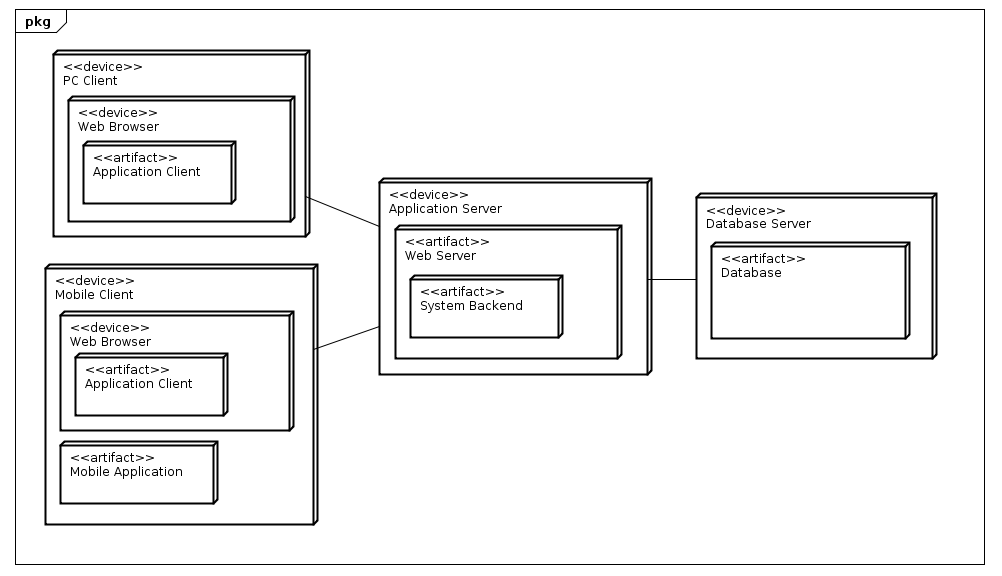
\includegraphics[width=\textwidth]{Images/UMLDiagrams/DeploymentDiagram.png}
\caption{Deployment Diagram}
\end{figure}

\clearpage